\section{Fase 9: Bitácora para el diagnóstico del cáncer de mama (BCDL) }
En esta fase, se propone el uso de una bitácora para el diagnóstico del cáncer de mama (BCDL, por sus siglas en inglés, \textit{“Breast Cancer Diagnostic Logbook”}). El propósito del \textit{BCDL} es almacenar las respuestas obtenidas por cada pregunta planteada en el \textit{BCQM} y la relación de estas preguntas y respuestas con determinado modelo de ML o DL. Esta bitácora solamente debe ser alimentada cuando la información obtenida generó valor agregado al dominio médico. Su principal propósito es evitar la redundancia de la información y la duplicidad de preguntas planteadas en el \textit{BCQM}, garantizando que en cada \textit{Release} se genere nuevo conocimiento relacionado al cáncer de mama. Se recomienda que la bitácora sea diseñada por medio de un \textit{modelo entidad relación (MER)} que este conformado por entidades como: modelo, tipo de cáncer de mama, técnica de diagnóstico, conjunto de datos, pregunta y respuesta. Dado lo anterior, se sugiere que los diferentes conjuntos de datos o imágenes utilizados en los análisis realizados, sean almacenados en un servicio de alojamiento en la nube (Amazon Cloud, Google Drive, One Drive, etc.) y que la información este identificada con un código único que facilite su búsqueda cuando sea requerido. De igual manera, los diferentes algoritmos generados deben ser almacenados en un sistema de control de versiones (GitLab, GitHub, Bitbucket, etc.) con su respectivo \textit{Readme} de funcionamiento y un código de identificación único para que pueda ser consultado fácilmente por base de datos. Por consiguiente, el uso del \textit{BCDL} permite tener una trazabilidad detallada de los avances obtenidos en cada \textit{Release} con respecto al diagnóstico del cáncer de mama, esto con el proposito de que el \textit{Data Analysis Team} tenga un punto de partida solido para innovar en nuevos modelos de ML y DL a través de la comparación y la mejora continua de modelos existentes que lograron agregar valor a los diferentes tipos de datos oncológicos.

\subsection{Modelo Entidad Relación (MER) para dominio oncológico}

Para este caso de estudio, el \textit{Modelo Entidad Relación (MER)} se desarrolló para facilitar el diseño de bases de datos basado en la especificación de un esquema para el diagnóstico del cáncer de mama para representar una estructura lógica global que permita ver la relación entre el investigador, el tipo de cáncer de mama, la técnica de diagnóstico, la técnica computacional, el lenguaje de programación  y la pregunta, respuesta y decisión médica. Dado lo anterior, el MER generado para el diagnóstico del cáncer de mama se puede observar en la figura \ref{MER}. De igual manera, en la tabla \ref{tablaMER} se describe cada entidad y su aplicación con el conjunto de datos analizado. 

%\newpage
\newgeometry{left=0.5cm, right=0.5cm, top=0.5cm, bottom=0.5cm}
\begin{landscape}
	\begin{figure}
		\centering
		\includegraphics[width=0.96
		\linewidth]{MER/IMAGENES_MER/0_MER_BCDL}
		\caption{Modelo Entidad Relación (MER) para el dominio oncológico enfocado en el diagnostico del cáncer de mama.}
		\label{MER}
	\end{figure}
\end{landscape}
\restoregeometry

\begin{table*}[htb!]
	\footnotesize
	\begin{threeparttable}
		\begin{tabular}{p{0.5cm} p{7cm} p{7cm}} \toprule 
			&\begin{center}Entidades y atributos\end{center}             
			&\begin{center}MER\end{center}\\ \hline
			1
			& La entidad \textit{Investigador} permite almacenar la información del \textit{Data Analysis Team}, el cual está conformado por el ingeniero de datos, el científico de datos y el medico oncólogo. Lo anterior con el propósito de crear una comunidad científica que permita poner en contacto a los investigadores para mejorar, aplicar y agilizar el diagnóstico del cáncer de mama. 
			& \begin{center}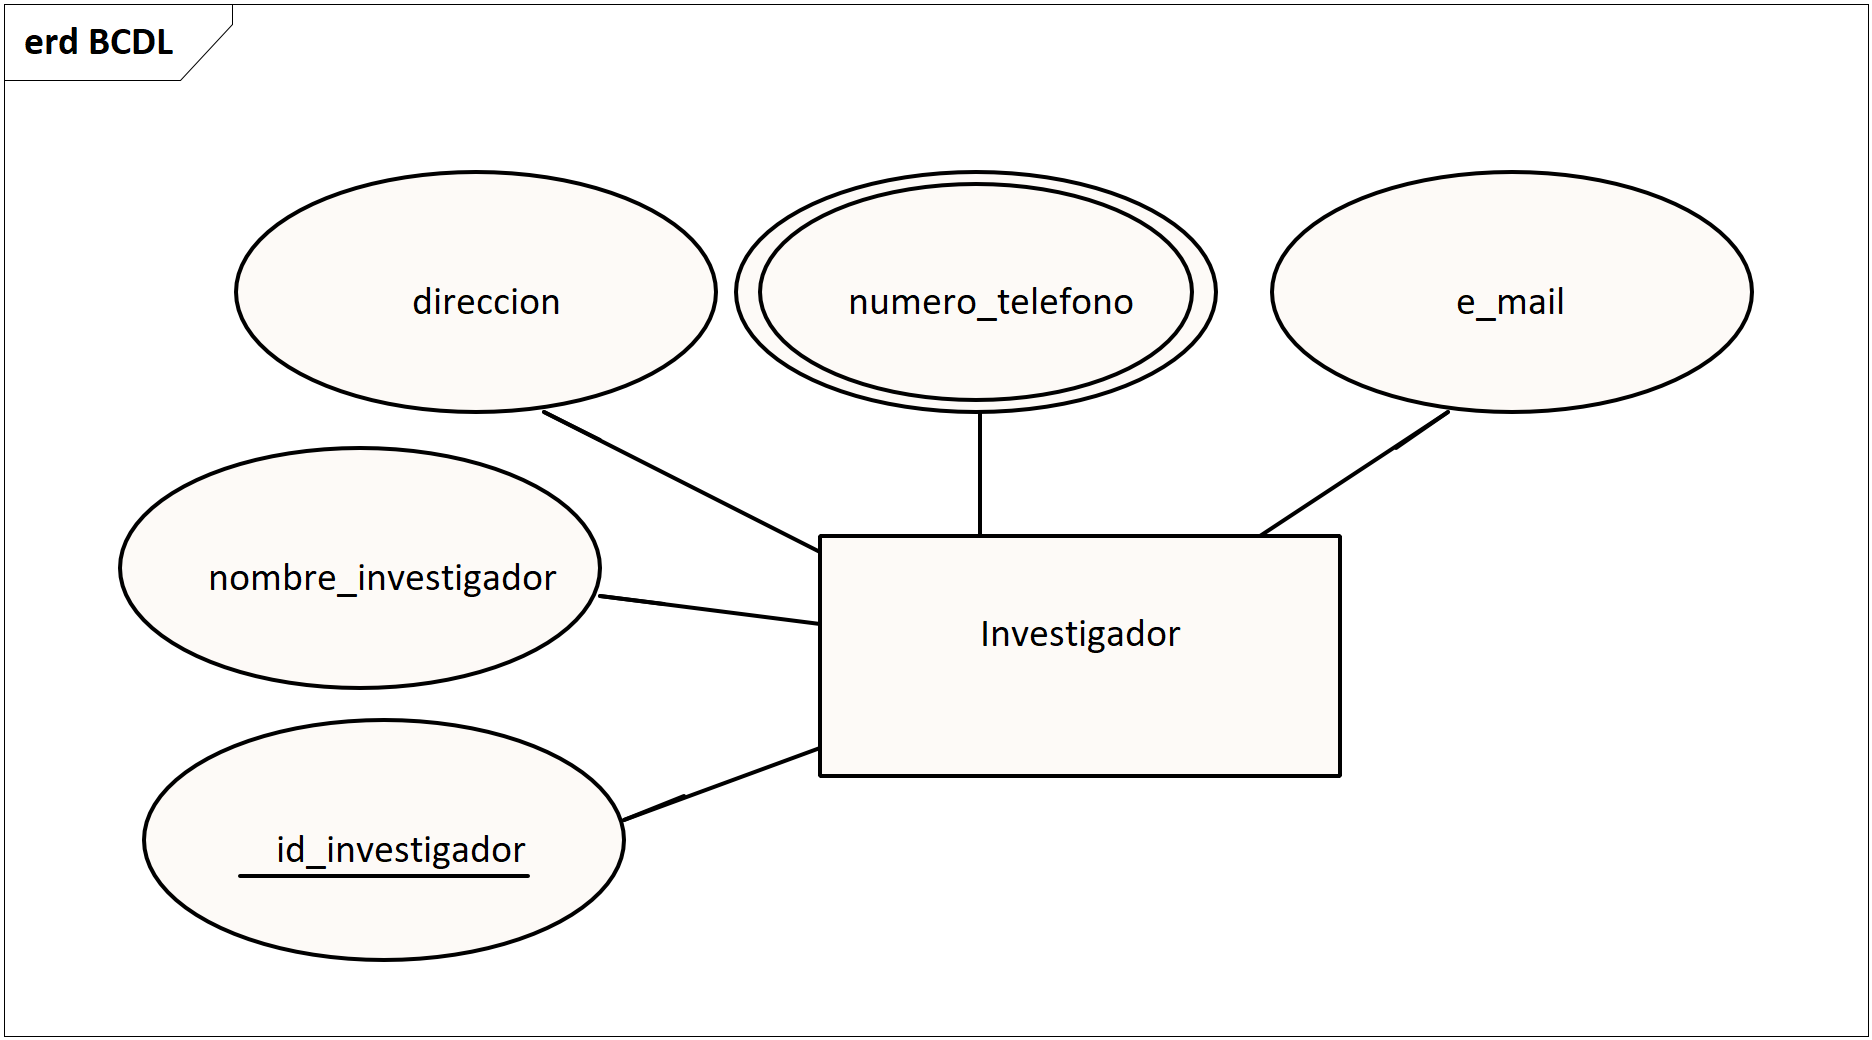
\includegraphics[width=1\linewidth]{MER/IMAGENES_MER/1_INVESTIGADOR}\end{center}
			\\ \hline
			%-----------------------------------------------------------
			2
			& La entidad \textit{Departamento} permite almacenar la información de las unidades de docencia e investigación del cáncer encargadas de coordinar las enseñanzas de varios ámbitos del conocimiento de acuerdo con la programación docente de la universidad. En este caso, nos permitirá conocer el enfoque (genética médica, oncología , genómica , epigramática, patología, etc.) de los investigadores involucrados en la aplicación de la ciencia de datos en el diagnóstico del cáncer de mama.
			& \begin{center}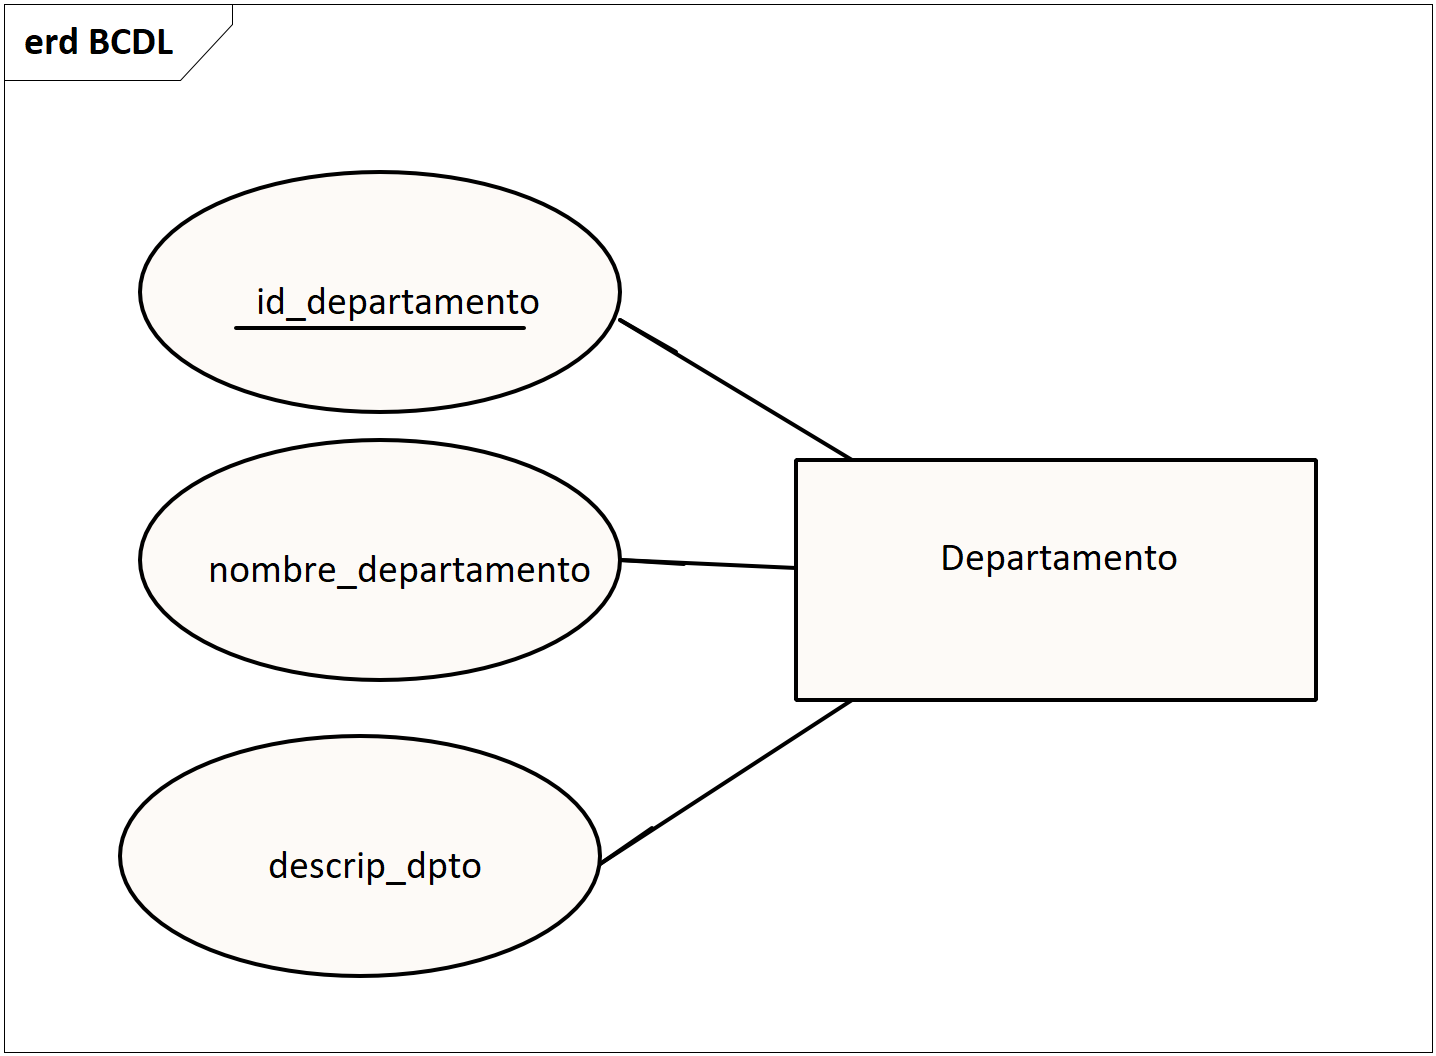
\includegraphics[width=1\linewidth]{MER/IMAGENES_MER/2_DEPARTAMENTO}\end{center}
			\\ \hline
			%-----------------------------------------------------------
			3
			& La entidad \textit{Universidad} permite almacenar la información de institución académica de enseñanza superior a la que está vinculado el investigador. Lo anterior, para conocer las fortalezas en la búsqueda de nuevos conocimiento e innovación con lo que respecta al diagnóstico del cáncer de mama.
			& \begin{center}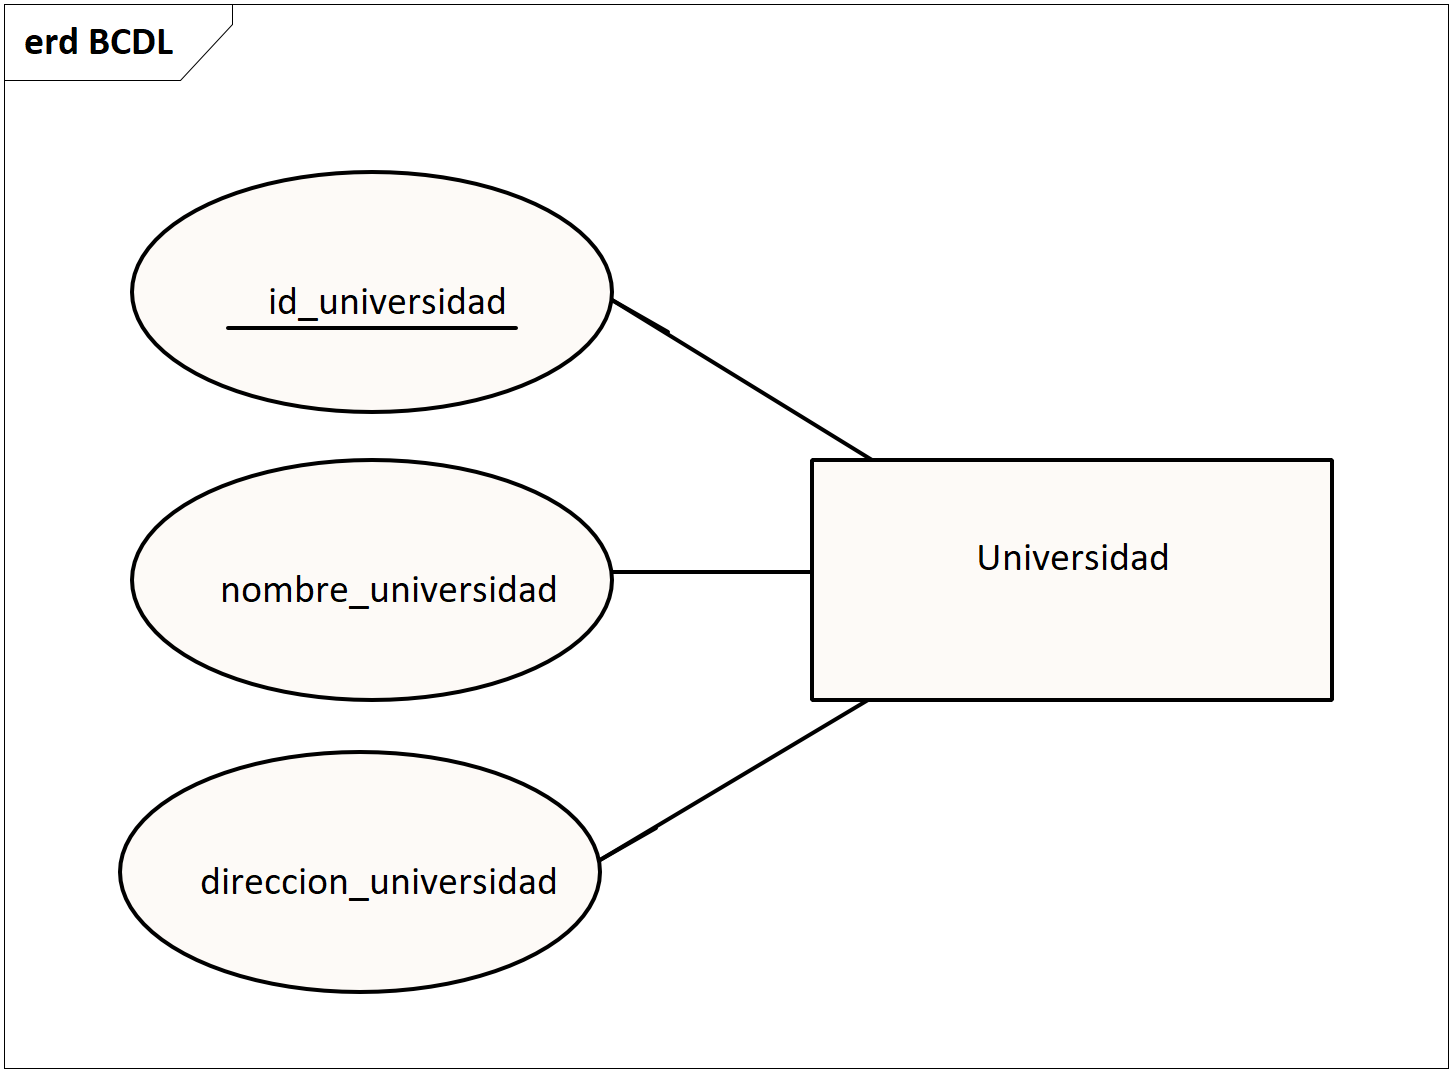
\includegraphics[width=1\linewidth]{MER/IMAGENES_MER/3_UNIVERSIDAD}\end{center}
			\\ \hline
			%-----------------------------------------------------------
			4
			& La entidad \textit{País} permite almacenar la ubicación geográfica de la universidad. Lo anterior, con el propósito de facilitar el contacto de los diferentes investigadores.
			& \begin{center}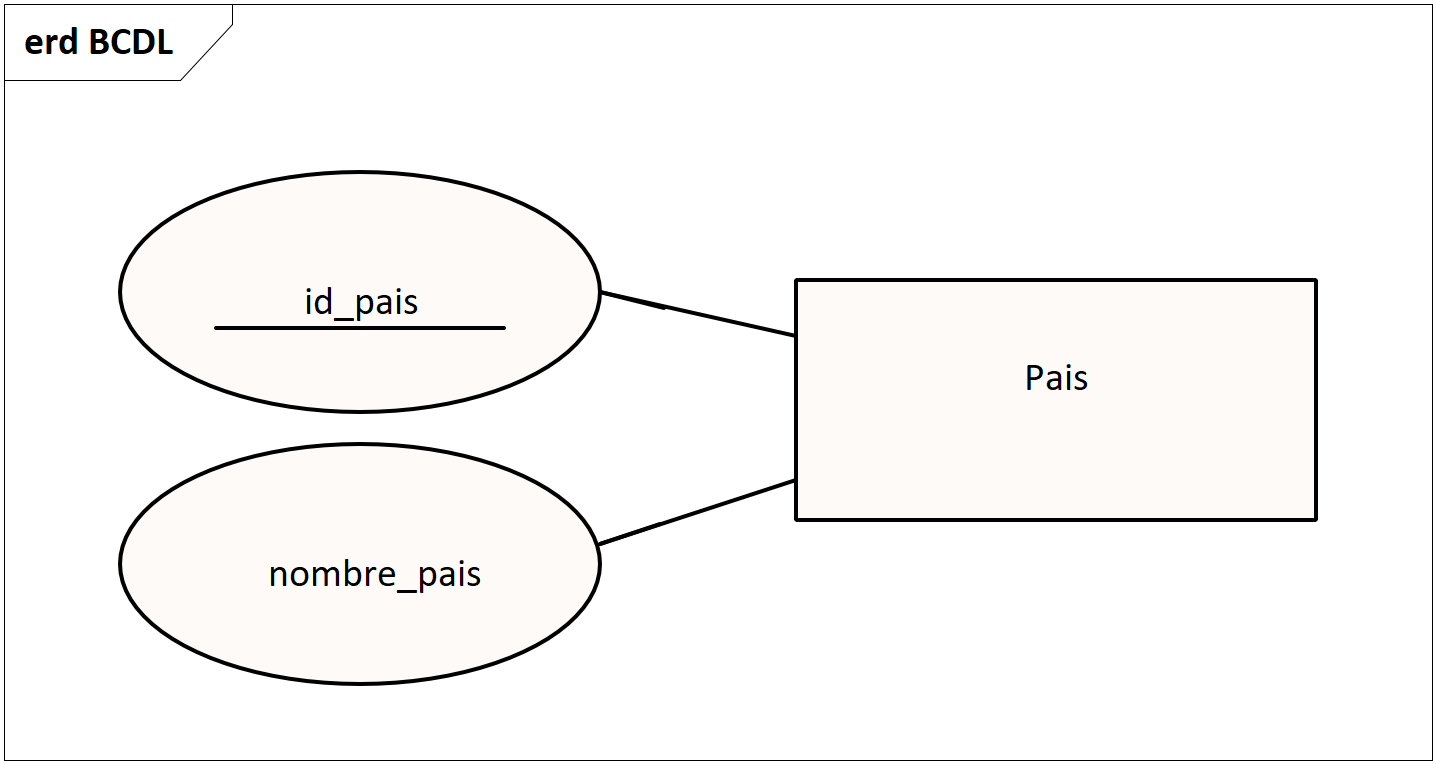
\includegraphics[width=1\linewidth]{MER/IMAGENES_MER/4_PAIS}\end{center}
			\\ \hline
		\end{tabular}
	\end{threeparttable}
\end{table*}

\begin{table*}[htb!]
	\footnotesize
	\begin{threeparttable}
		\begin{tabular}{p{0.5cm} p{7cm} p{7cm}} \toprule 
			5
			& La entidad \textit{Pregunta} permite almacenar la información de las preguntas que fueron resueltas al finalizar un \textit{Release} y que están relacionadas con el tipo de cáncer de mama, la técnica de diagnóstico y un conjunto de datos determinado. 
			& \begin{center}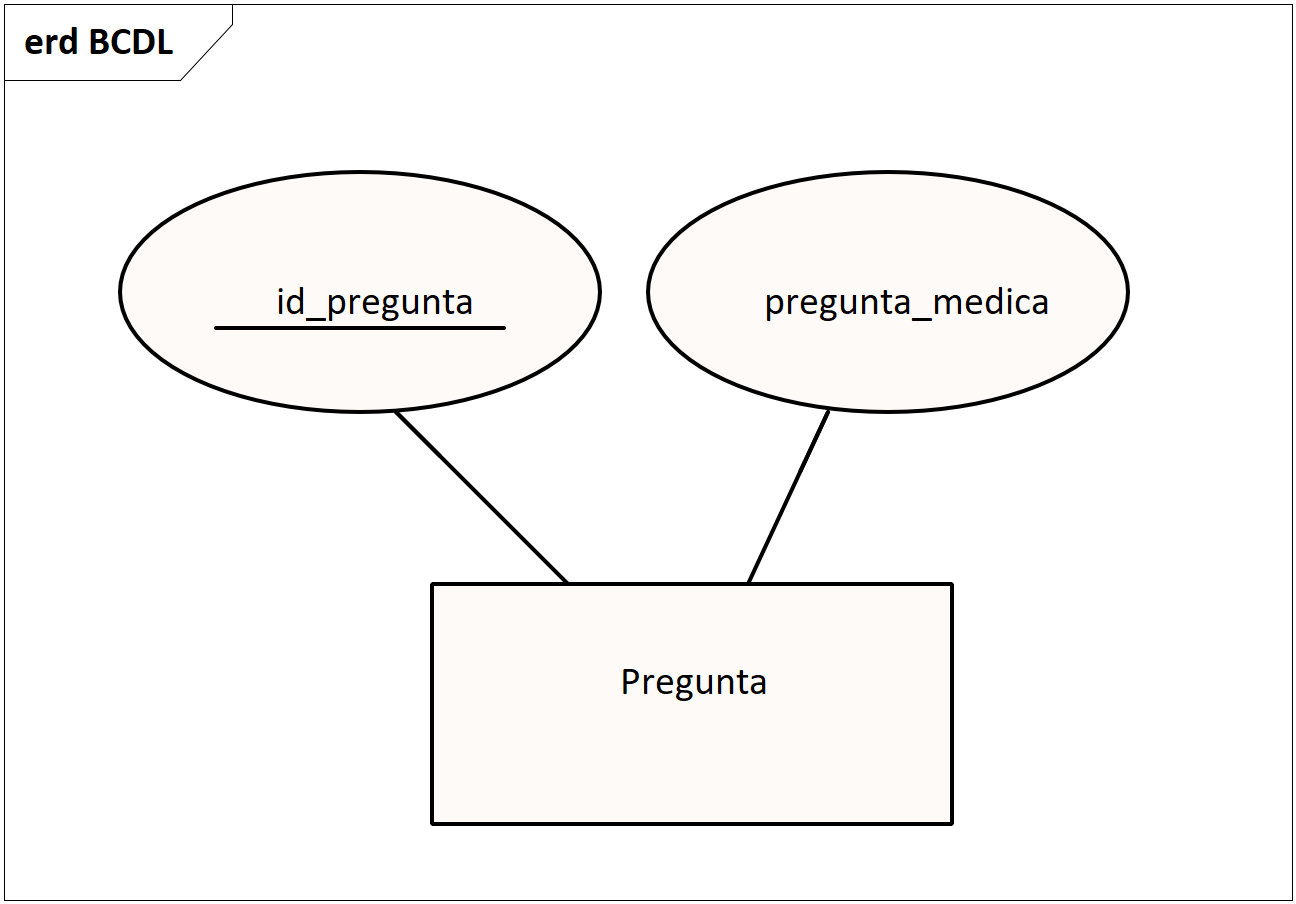
\includegraphics[width=1\linewidth]{MER/IMAGENES_MER/5_PREGUNTA}\end{center}
			\\ \hline
			%-----------------------------------------------------------
			6
			& La entidad \textit{Respuesta} permite almacenar la información de las respuestas obtenidas al finalizar un \textit{Release} y que servirán para que el oncólogo tome decisiones medicas con respecto al diagnóstico del cáncer de mama.
			& \begin{center}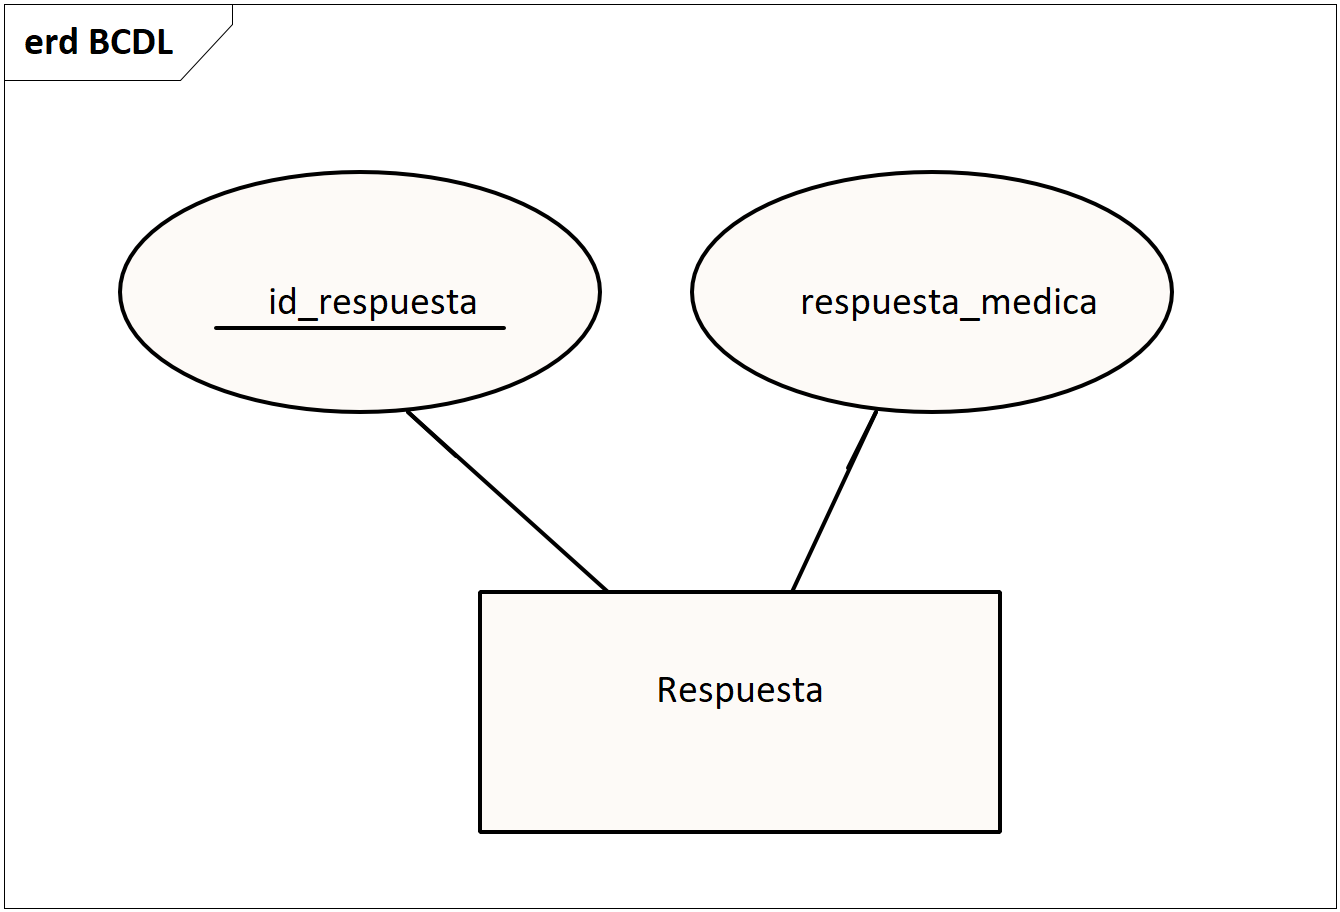
\includegraphics[width=1\linewidth]{MER/IMAGENES_MER/6_RESPUESTA}\end{center}
			\\ \hline
			%-----------------------------------------------------------
			7
			& La entidad \textit{Decisión} permite almacenar la información de las decisiones generados por el especialista en oncología. Lo anterior, para garantizar que los resultados obtenidos permitan diagnosticar de una manera ágil el posible padecimiento de cáncer de mama y así generar un tratamiento oportuno.
			& \begin{center}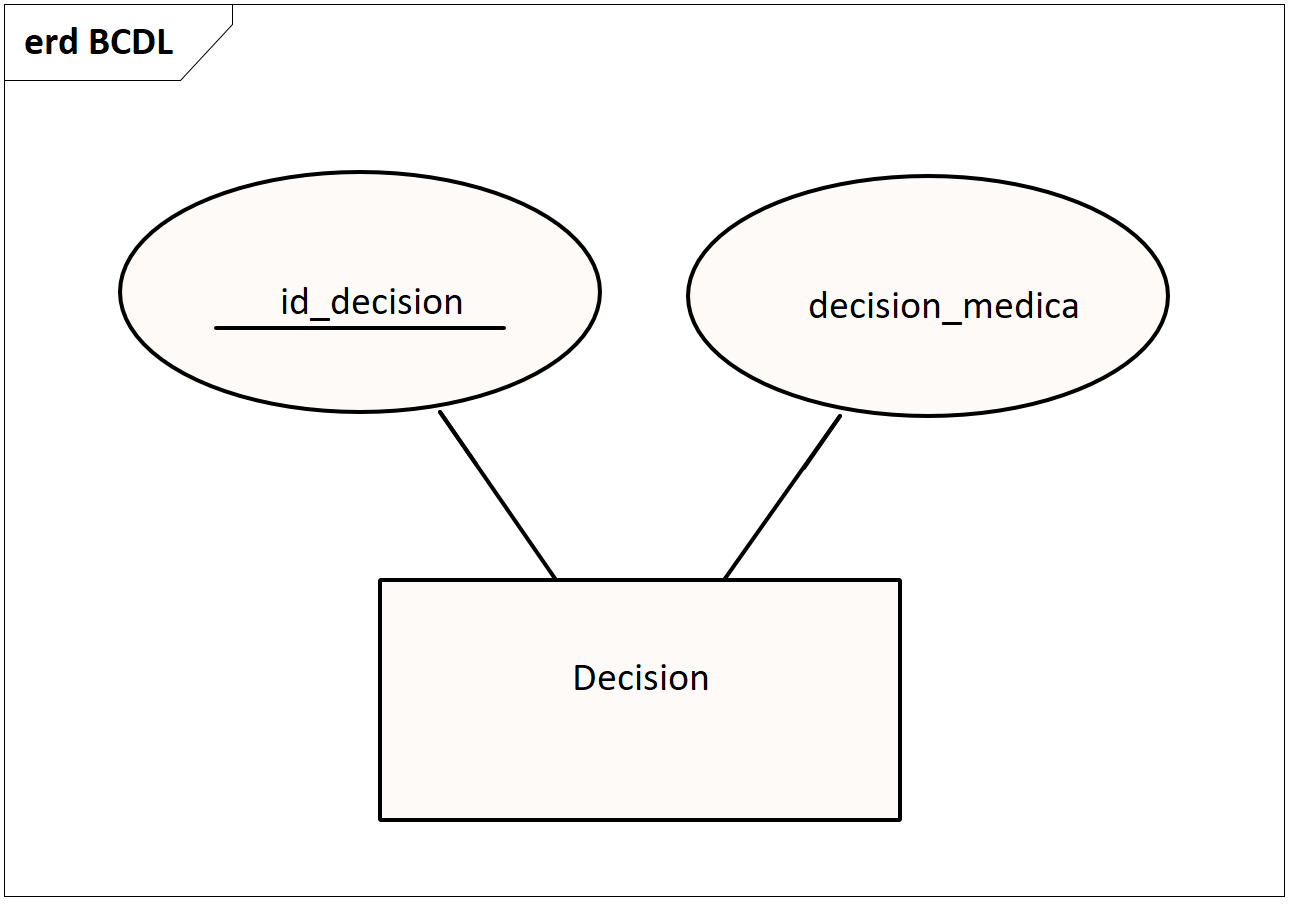
\includegraphics[width=1\linewidth]{MER/IMAGENES_MER/7_DECISION}\end{center}
			\\ \hline
			%-----------------------------------------------------------
			8
			& La entidad \textit{Cáncer de seno} permite almacenar el grupo de carcinoma de mama al que está orientado el análisis de datos. En este caso, los grupos más conocidos son: Carcinoma ductal in situ de mama (CDIS), 
			Neoplasias fibroepiteliales de mama (BFN), Sarcoma de mama (SBP), Carcinoma invasivo de mama (BRCA) y Carcinoma de mama metaplásico (CMM).
			& \begin{center}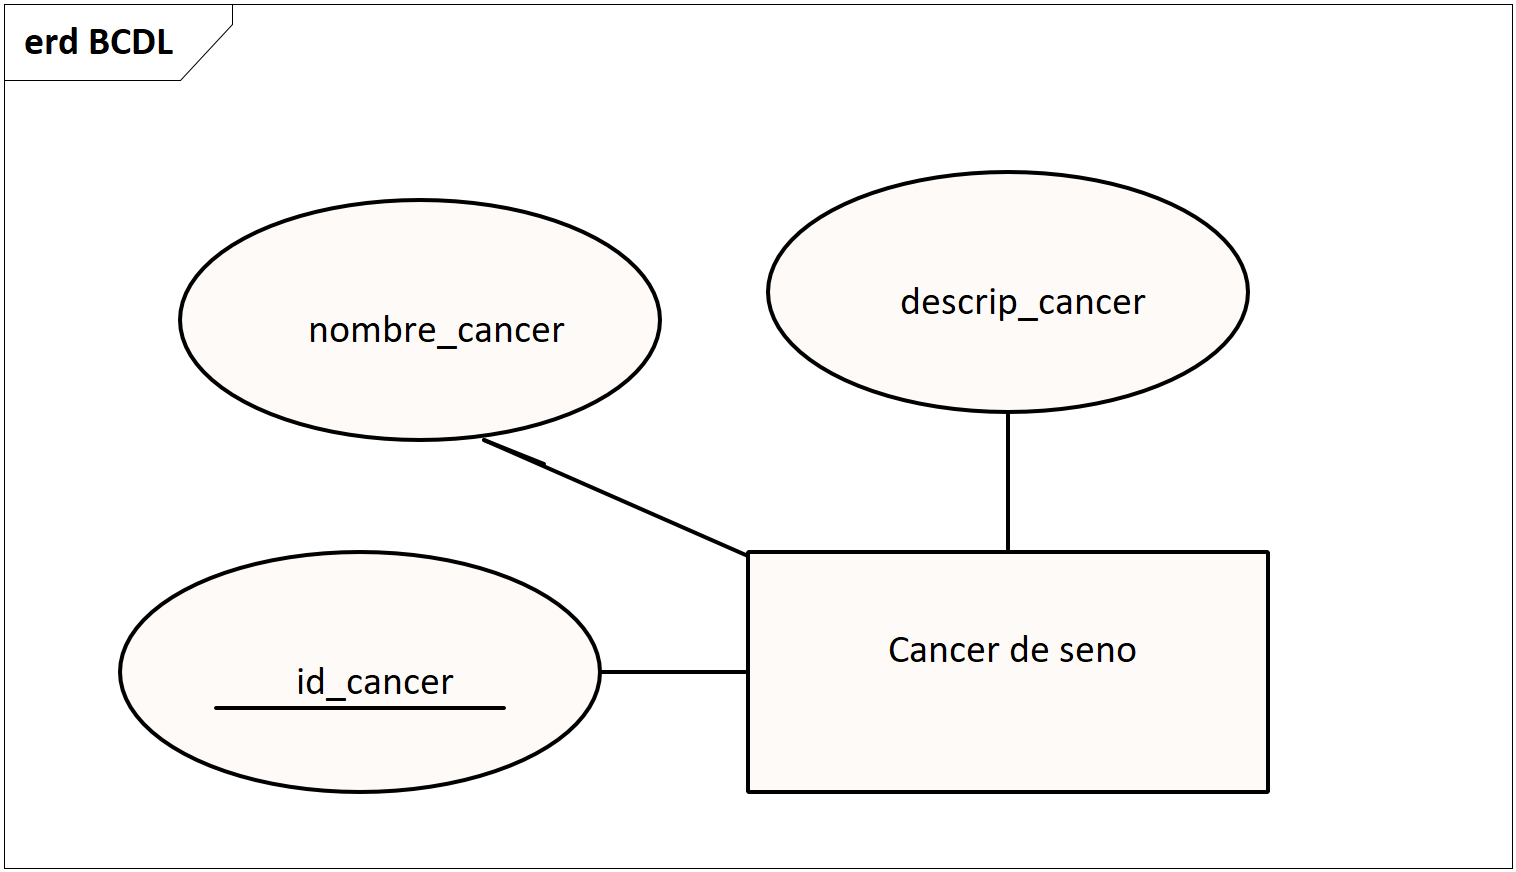
\includegraphics[width=1\linewidth]{MER/IMAGENES_MER/8_CANCER}\end{center}
			\\ \hline
		\end{tabular}
	\end{threeparttable}
\end{table*}

\begin{table*}[htb!]
	\footnotesize
	\begin{threeparttable}
		\begin{tabular}{p{0.5cm} p{7cm} p{7cm}} \toprule 
			9
			& La entidad \textit{Tipo de cáncer} permite almacenar la información del tipo de carcinoma de mama al que está orientado el análisis de datos.  En este caso, los tipos más conocidos son: Adenomioepitelioma de mama (BRAME), Carcinoma lobulillar in situ de mama (LCIS), Neoplasia mamaria NOS (BNNOS), Cáncer de mama inflamatorio (IBC) y Carcinoma secretor juvenil de mama (JSCB).
			& \begin{center}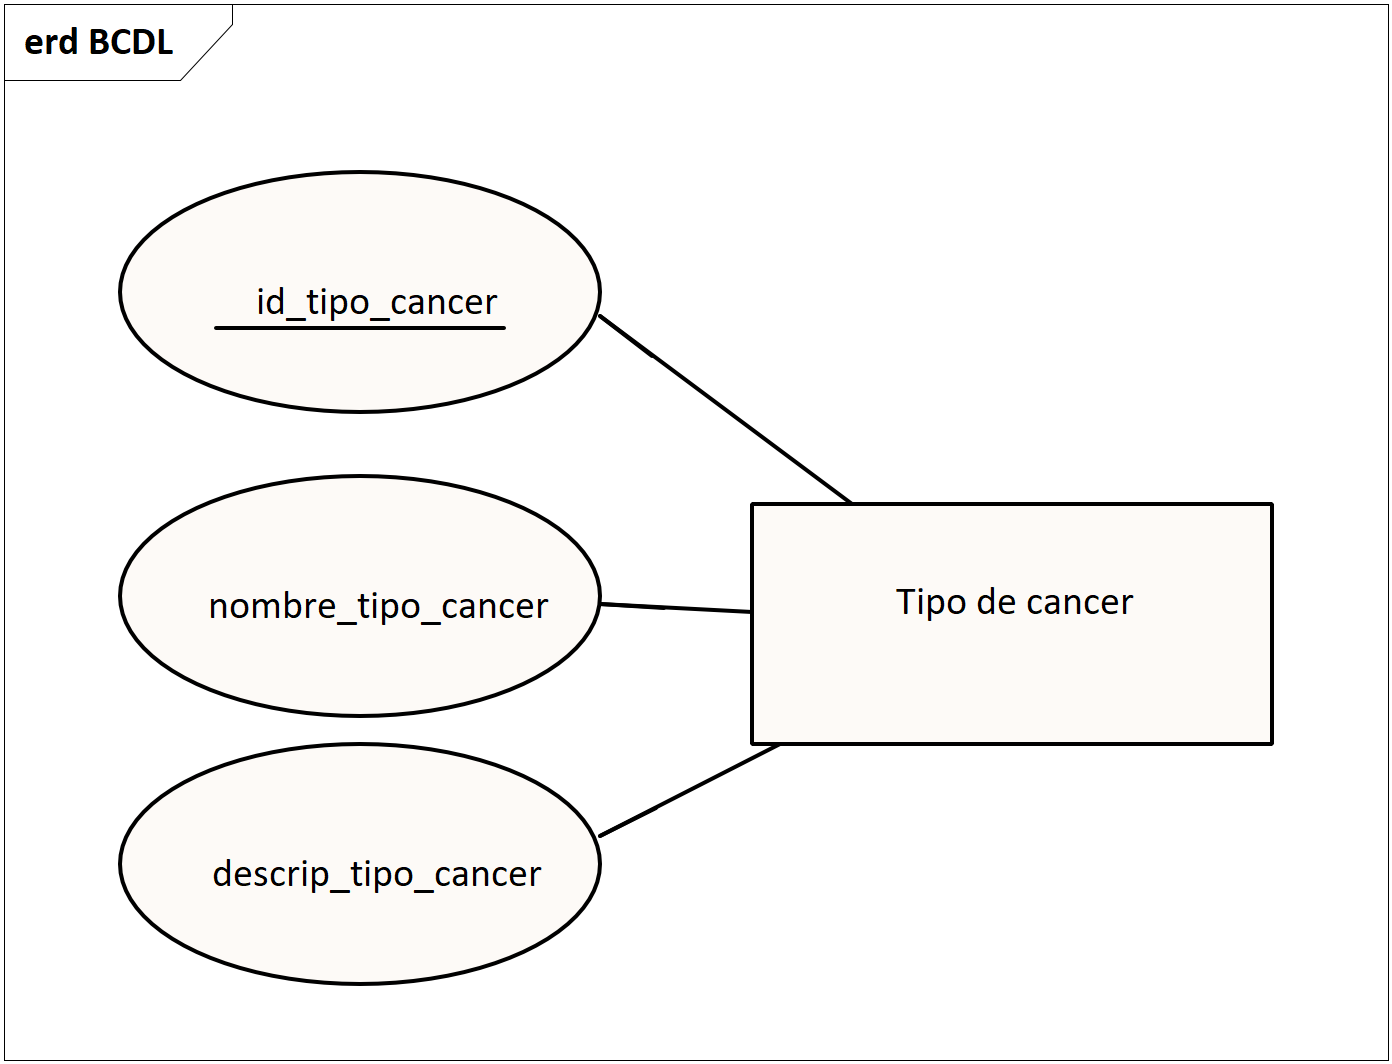
\includegraphics[width=1\linewidth]{MER/IMAGENES_MER/9_TIPO_CANCER}\end{center}
			\\ \hline
			%-----------------------------------------------------------
			10
			& La entidad \textit{Sub-tipo de cáncer} permite almacenar la información del sub-tipo de carcinoma de mama al que está orientado el análisis de datos. En este caso, los sub-tipos más conocidos son: Enfermedad de Paget del pezón (PD), Fibroadenoma (FA), Tumor filoides de mama (PT), Angiosarcoma de mama (BA), Carcinoma ductal y lobulillar mixto de mama (MDLC), Carcinoma mucinoso mixto invasivo de mama (IMMC), Carcinoma mucinoso mixto invasivo de mama (IMMC), Carcinoma lobular invasivo (ILC), Carcinoma ductal invasivo de mama (IDC), Carcinosarcoma invasivo de mama, NOS (CSNOS), Carcinoma invasivo de mama, NOS (BRCNOS), Carcinoma de mama con anillo de sello (BRSRCC), cáncer de mama adenoide quístico (ACBC), carcinoma papilar sólido de mama (SPC), cáncer de mama metaplásico de tipo epitelial (EMBC) y cáncer de mama metaplásico de tipo mixto (MMBC)
			& \begin{center}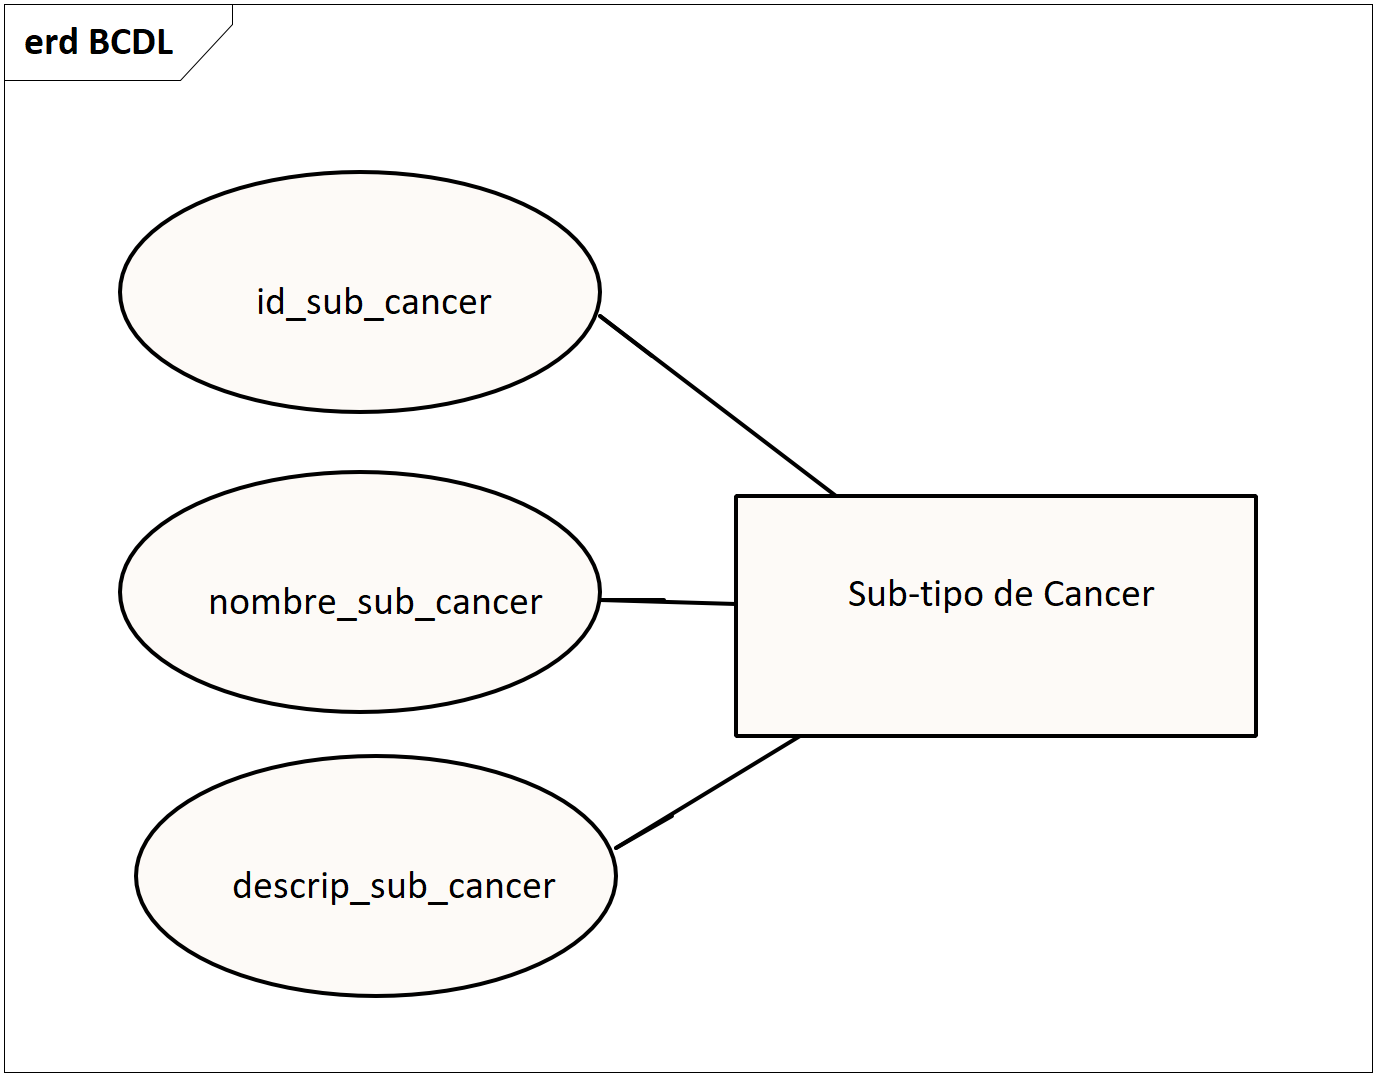
\includegraphics[width=1\linewidth]{MER/IMAGENES_MER/10_SUBTIPO_CANCER}\end{center}
			\\ \hline
			%-----------------------------------------------------------
			11
			& La entidad \textit{Técnica de diagnóstico} permite almacenar la informacion la técnica utilizada para el diagnóstico del cáncer de mama. En este caso, las técnicas más conocidas son: mamografía, ductografía, ecografía, Resonancia Magnética (MRI), biopsia por aspiración con aguja fina (FNA) y biopsia con aguja gruesa (CNB).
			& \begin{center}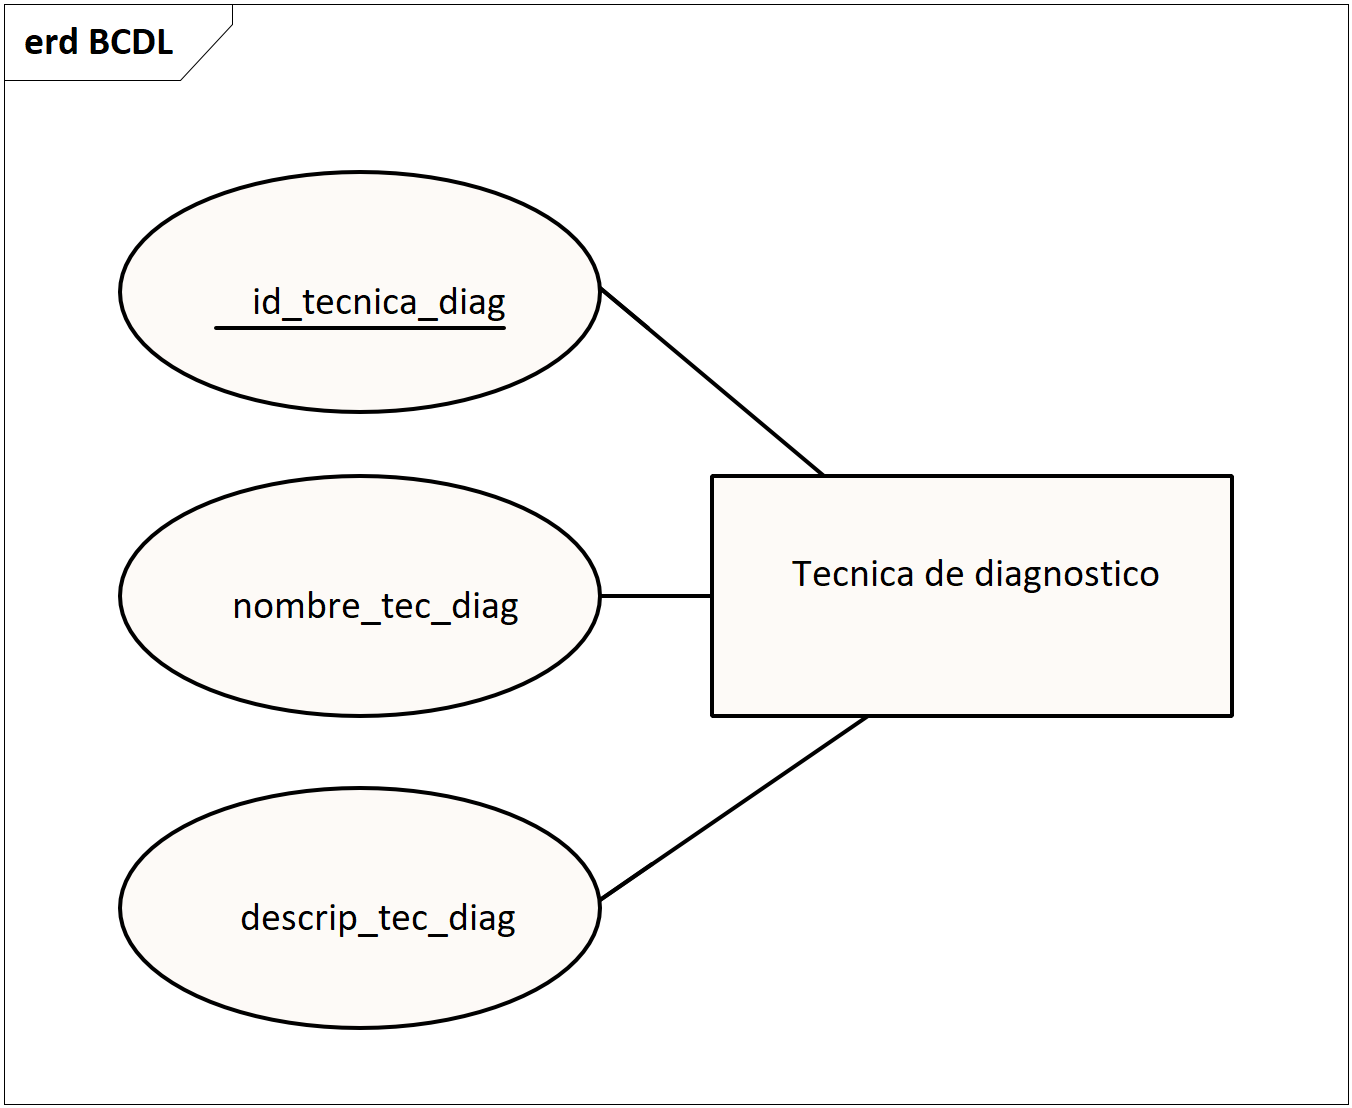
\includegraphics[width=1\linewidth]{MER/IMAGENES_MER/11_TECNICA_DIAGNOSTICO}\end{center}
			\\ \hline
			%-----------------------------------------------------------
		\end{tabular}
	\end{threeparttable}
\end{table*}

\begin{table*}[htb!]
	\footnotesize
	\begin{threeparttable}
		\begin{tabular}{p{0.5cm} p{7cm} p{7cm}} \toprule 
			12
			& La entidad \textit{Conjunto de datos} permite almacenar la información del conjunto de datos que fue obtenido a través del tipo de cáncer de mama y la técnica de diagnóstico. Lo anterior, con el propósito de identificar la ubicación del repositorio en la nube, la cantidad, el tamaño y el tipo de registros procesados por el algoritmo de ML o DL relacionado a una técnica computacional. 
			
			& \begin{center}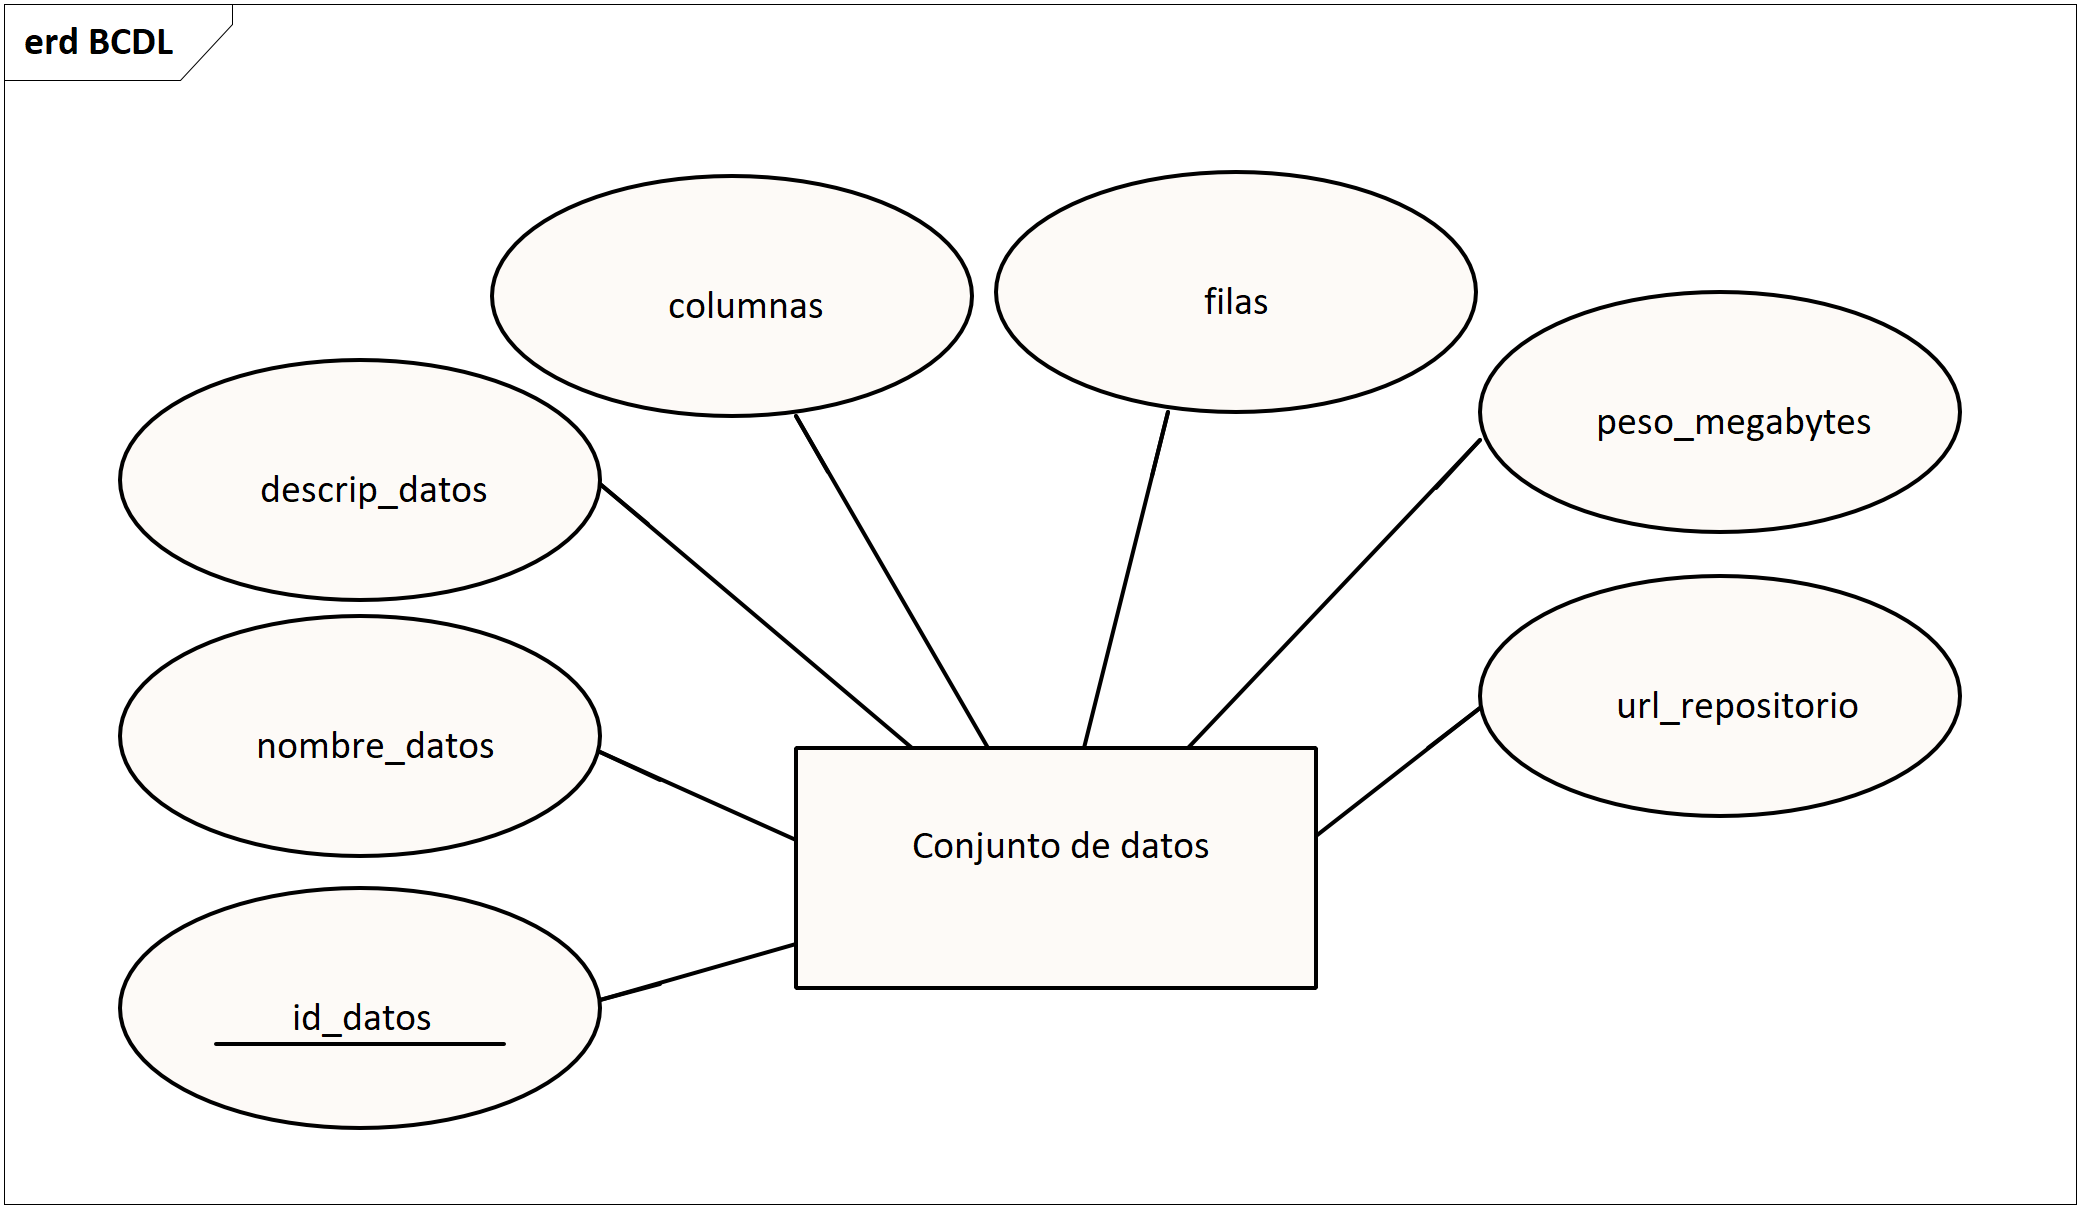
\includegraphics[width=1\linewidth]{MER/IMAGENES_MER/12_CONJUNTO_DATOS}\end{center}
			\\ \hline
			%-----------------------------------------------------------
			13
			& La entidad \textit{Técnica Computacional} permite almacenar la información de la técnica de aprendizaje automático utilizada con un conjunto determinado de datos. En este caso, las técnicas computacionales más conocidas son: clasificación, agrupamiento, regresión, redes neuronales y reducción dimensional. 
			& \begin{center}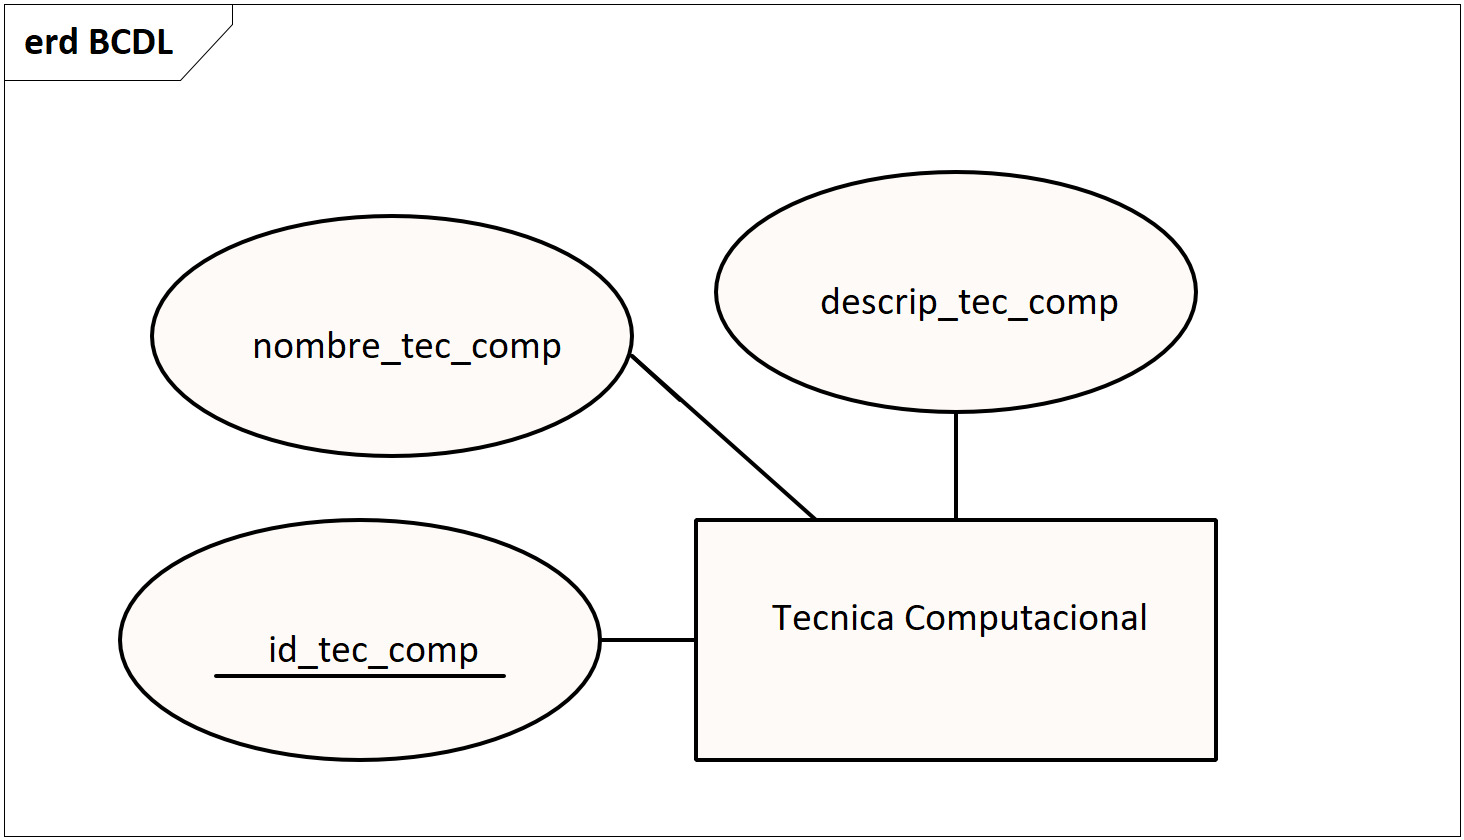
\includegraphics[width=1\linewidth]{MER/IMAGENES_MER/13_TECNICA_COMPUTACIONAL}\end{center}
			\\ \hline
			%-----------------------------------------------------------
			14
			& La entidad \textit{Modelo} permite almacenar la información del modelo de ML o DL utilizado para ser entrenado con un conjunto determinado de datos. En este caso, los modelos más conocidos son: regresión lineal, regresión logística, arboles de decisión, bosque aleatorio, K-means, K-modes, BIRCH y redes neuronales convolucionales.
			& \begin{center}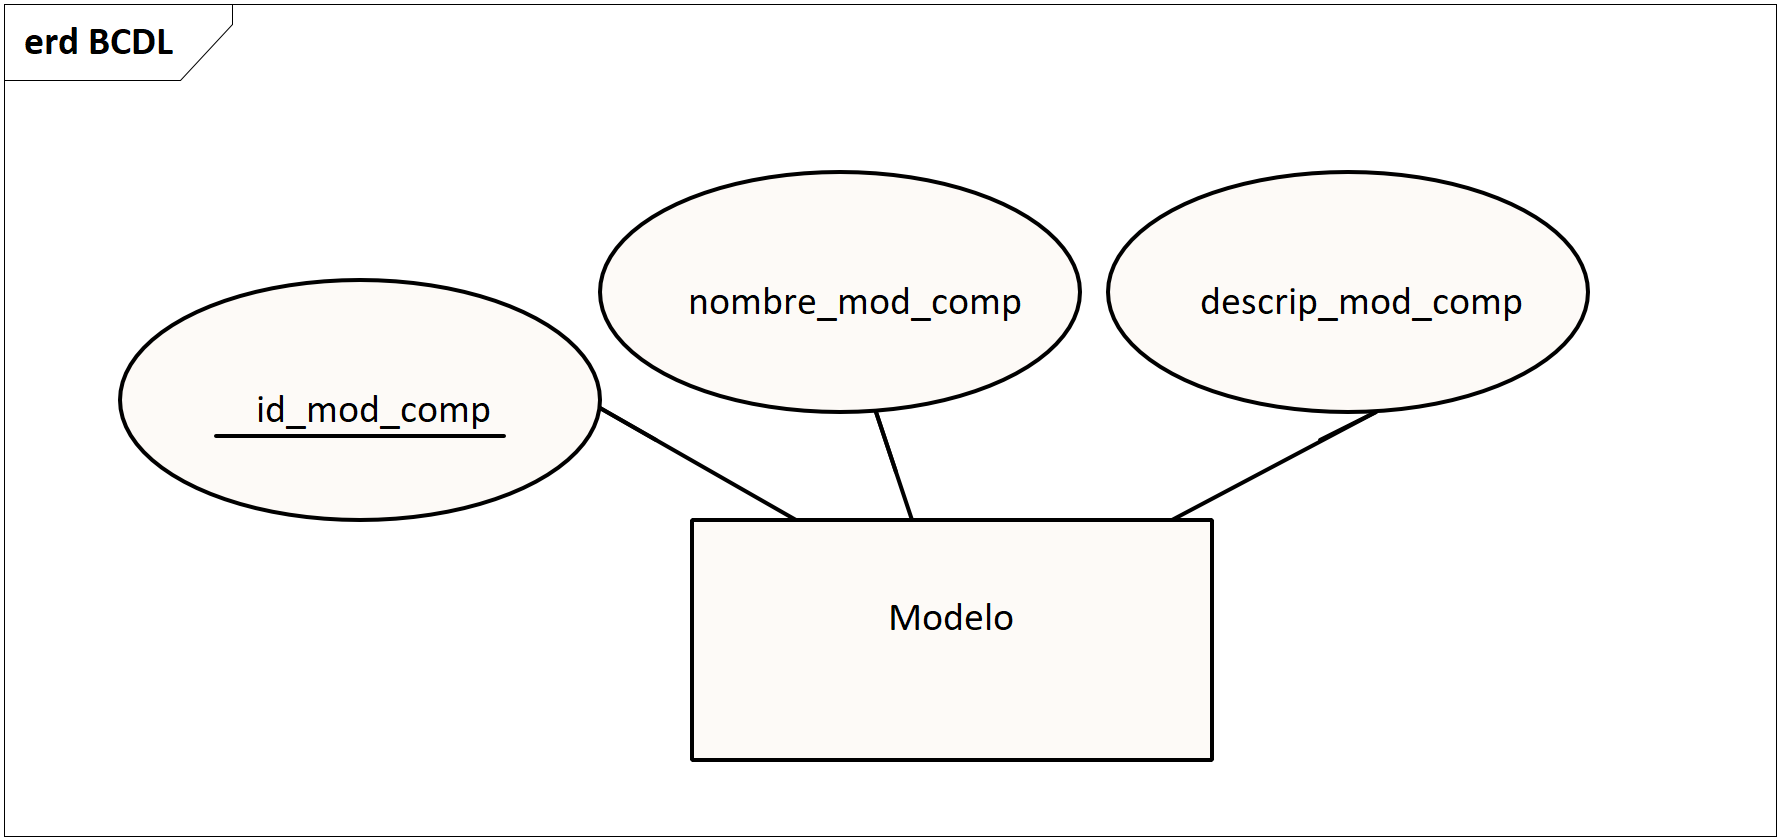
\includegraphics[width=1\linewidth]{MER/IMAGENES_MER/14_MODELO}\end{center}
			\\ \hline
			%-----------------------------------------------------------
			15
			& La entidad \textit{Algoritmo} permite almacenar la información de la secuencia de pasos utilizados para ejecutar el modelo de ML o DL con el conjunto de datos basado en el diagnóstico del cáncer de mama. Lo anterior, con el propósito de identificar la ubicación del repositorio en la nube y la precisión del algoritmo. Cabe resaltar, que el objetivo principal de esta entidad es que los algoritmos tengan una mejora continua según la retroalimentación medica generada por el experto en oncología.
			& \begin{center}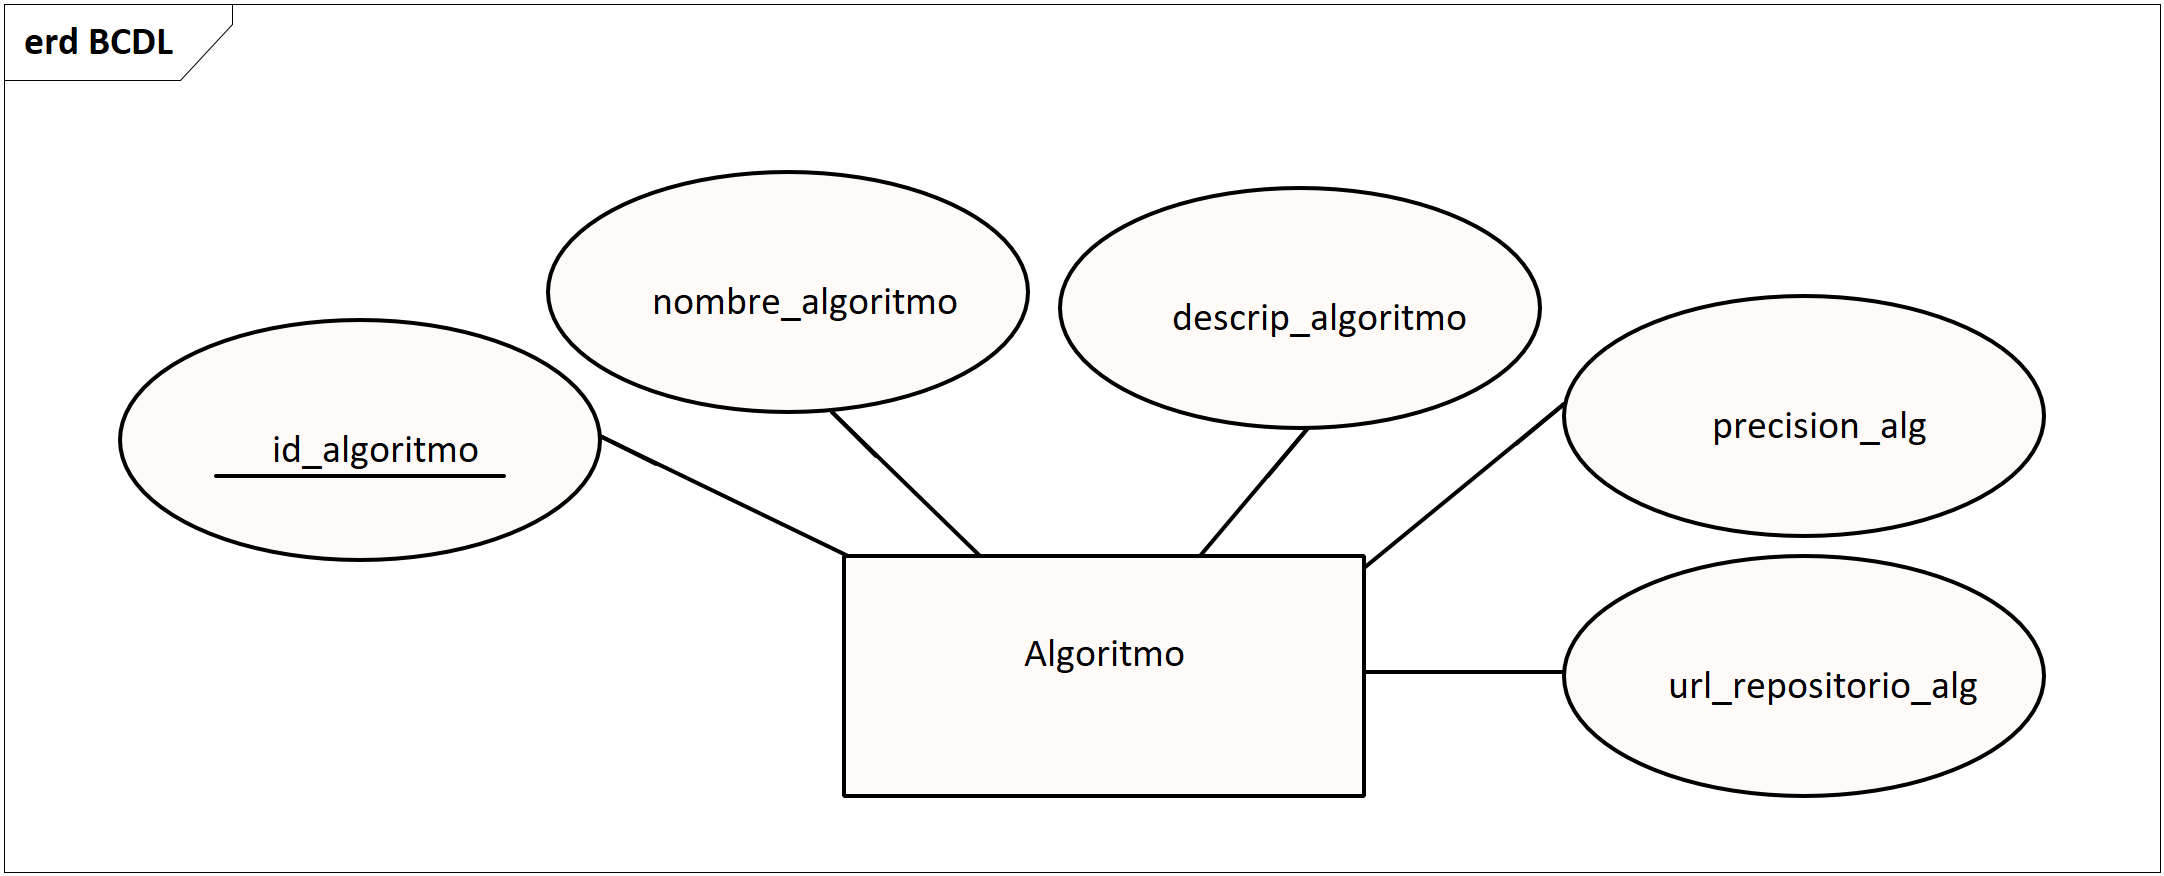
\includegraphics[width=1\linewidth]{MER/IMAGENES_MER/15_ALGORITMO}\end{center}
			\\ \hline
			%-----------------------------------------------------------
		\end{tabular}
	\end{threeparttable}
\end{table*}
\begin{table*}
	\footnotesize
	\begin{threeparttable}
		\begin{tabular}{p{0.5cm} p{7cm} p{7cm}} \toprule 
			16
			& La entidad \textit{Librería} permite almacenar la información del conjunto de implementaciones funcionales codificadas en un lenguaje de programación determinado. Lo anterior, con el propósito de identificar la documentación, versión y las propiedades de la librería utilizada para agilizar la implementación algorítmica de la ejecución de los modelos de ML y DL en pro de obtener resultados que generen valor de los datos obtenidos a través de las técnicas para el diagnóstico del cáncer de mama. En este caso, las librerías más conocidas son: Pandas, Numpy, Plotly, Scikit Learn, Keras y Tensorflow.
			
			& \begin{center}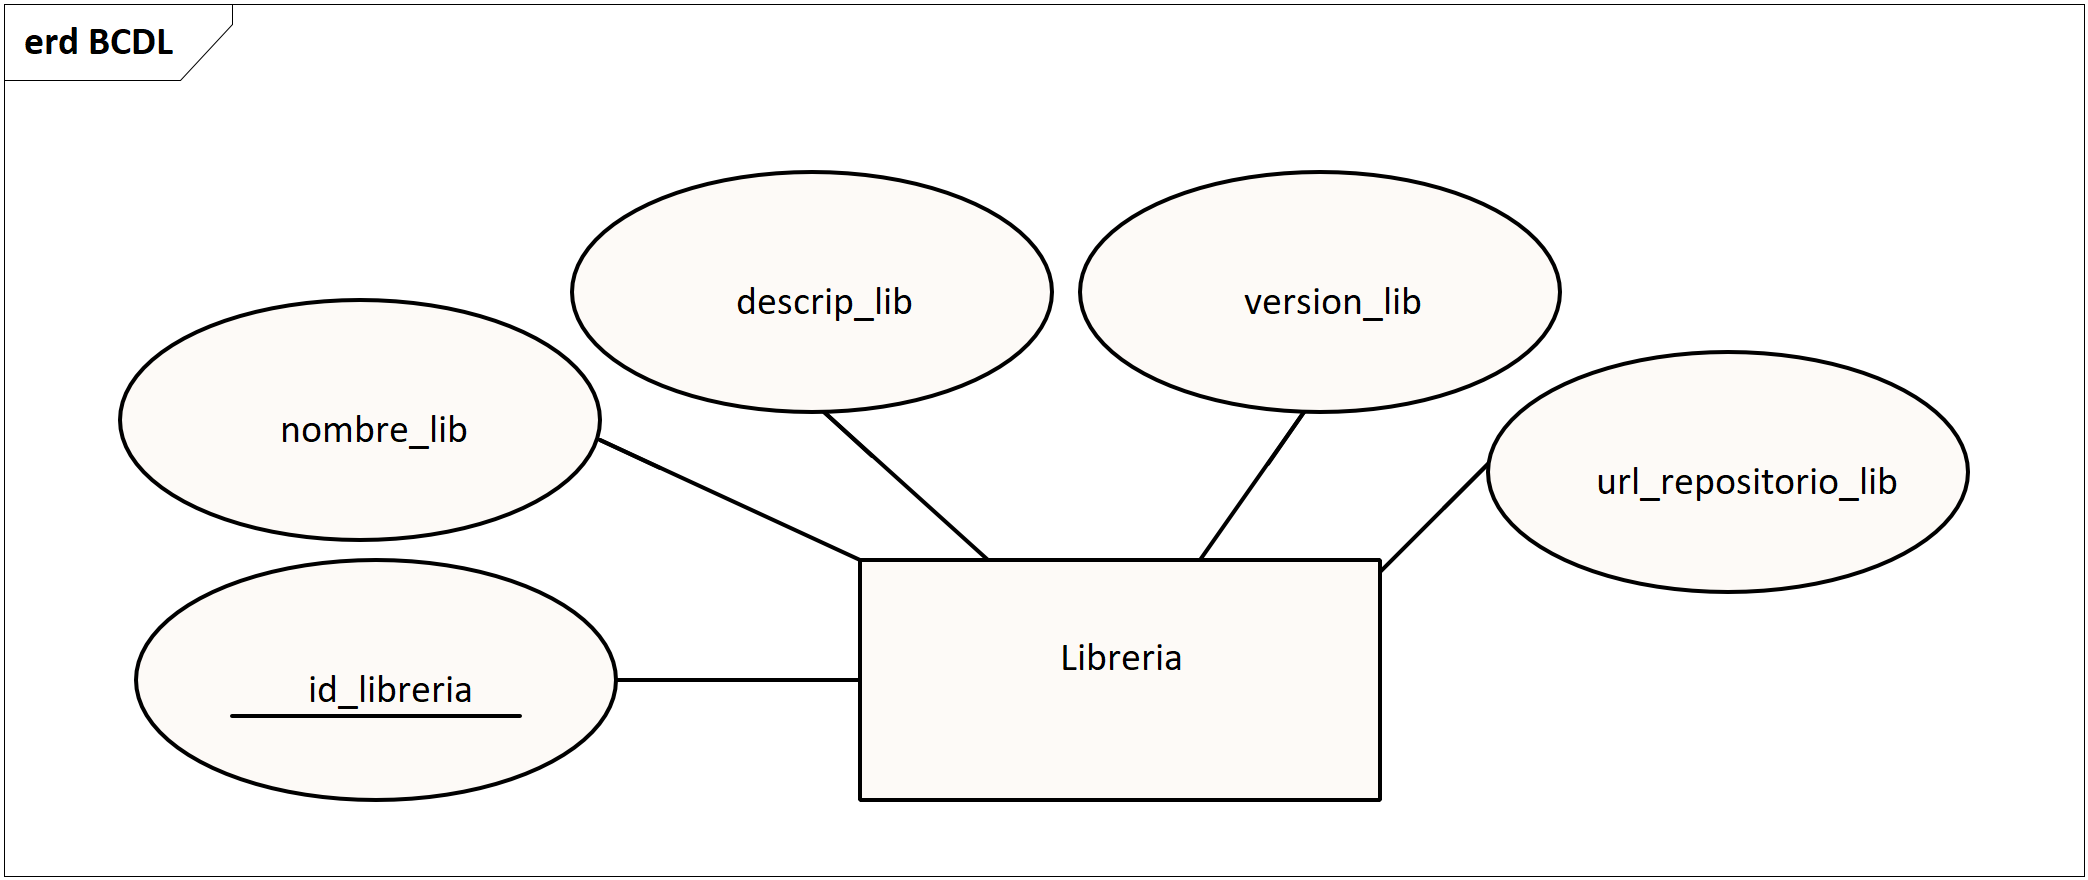
\includegraphics[width=1\linewidth]{MER/IMAGENES_MER/16_LIBRERIA}\end{center}
			\\ \hline
			%-----------------------------------------------------------
			17
			& La entidad \textit{Lenguaje de Programación} permite almacenar la información del lenguaje de programación y la versión utilizada para importar las librerías y garantizar el desempeño de la depuración de los algoritmos implementados con base a la ejecución de los modelos de ML y DL en pro de obtener resultados que generen valor de los datos obtenidos a través de las técnicas para el diagnóstico del cáncer de mama. En este caso, los lenguajes de programación más conocidos son: Python, R, SQL, Java, Scala, Julia y Matlab.  
			& \begin{center}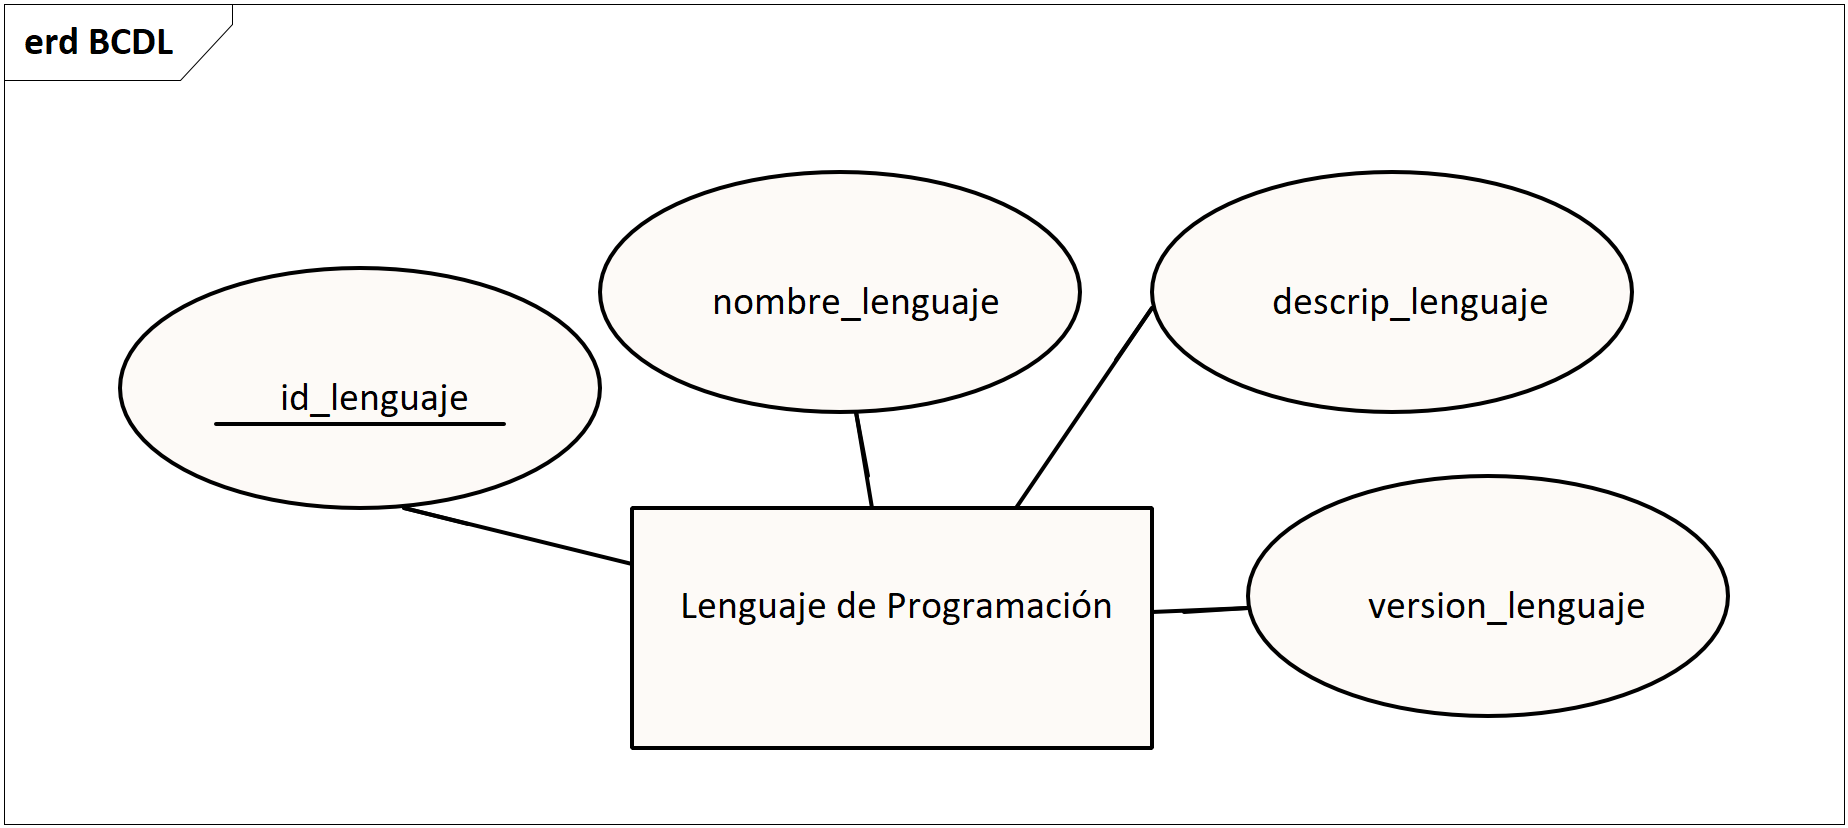
\includegraphics[width=1\linewidth]{MER/IMAGENES_MER/17_LENGUAJE_PROGRAMACION}\end{center}
			\\ \hline
			%-----------------------------------------------------------
		\end{tabular}
		\caption{Entidades y atributos para el dominio oncológico enfocado en el diagnóstico del cáncer de mama.}
		\label{tablaMER}
	\end{threeparttable}
\end{table*}
